\documentclass[a4paper, 12pt]{article}


\usepackage[english]{babel}
\usepackage[utf8]{inputenc}
\usepackage{graphicx}
\usepackage[a4paper, width=150mm, top=25mm, bottom=25mm]{geometry}
\usepackage{mathptmx}
\usepackage[T1]{fontenc}
\usepackage{enumitem}
\usepackage{amsmath}
\usepackage{index}
\usepackage{fancyhdr}
\usepackage{titlesec}
\usepackage{subfig}
\usepackage{listings}
\usepackage{listings-rust}
\titleformat{\chapter}{\normalfont\huge}{\thechapter.}{20pt}{\huge\it}



\usepackage{biblatex}
\addbibresource{containerized.bib}

\graphicspath{ {./programming_symbols/} }

\usepackage{listings}
\usepackage{xcolor}

\definecolor{codegreen}{rgb}{0,0.6,0}
\definecolor{codegray}{rgb}{0.5,0.5,0.5}
\definecolor{codepurple}{rgb}{0.58,0,0.82}
\definecolor{backcolour}{rgb}{0.95,0.95,0.92}

\lstdefinestyle{mystyle}{
    backgroundcolor=\color{backcolour},   
    commentstyle=\color{codegreen},
    keywordstyle=\color{magenta},
    numberstyle=\tiny\color{codegray},
    stringstyle=\color{codepurple},
    basicstyle=\ttfamily\footnotesize,
    breakatwhitespace=false,         
    breaklines=true,                 
    captionpos=b,                    
    keepspaces=true,                 
    numbers=left,                    
    numbersep=5pt,                  
    showspaces=false,                
    showstringspaces=false,
    showtabs=false,                  
    tabsize=2
}


\usepackage{hyperref}
\hypersetup{
    colorlinks=true,
    linkcolor=blue,
    filecolor=magenta,      
    urlcolor=cyan,
}

\urlstyle{same}
\lstset{style=mystyle}



\begin{document}
\title{\Large{\textbf{DBD Exam Report}}}
\author{Henning W.}
\date{\today}
\maketitle
\fancyhf{}
\renewcommand{\headrulewidth}{2pt}
\renewcommand{\headrulewidth}{2pt}
\fancyhead{\leftmark}
\fancyfoot{\thepage}

\section{Target Audience}
This report was not written to cater to all audiences. It is meant to be some sort of set of instructions, explanations and guidelines of the architecture of the program. It seldomly goes into detail about what the terminology means.  

\section{Introduction}
This project involves a simulation of some of the features of a social media platform. Due to time constraints, many of the features I usually would be using in my setup, has been skipped entirely to meet the deadline. This includes serving the applications in the cloud, CI/CD, logging and proper documentation (Sphinx and Rustdoc in this project).

Since the assignment definition states a requirement for large amounts of data, the project has been created a bit backwards. I've looked at some datasets, and then formulated data models from them. This of course also has an effect on how meaningful the data is. The project is thoroughly tested throughout multiple machines, owned by multiple people with different operating systems. 

The project's repository can be found here: 
\url{https://github.com/Mutestock/dbd\_exam}

\section{Installation}
Open a terminal in the project's directory. Then:

\begin{lstlisting}[language=Rust]
docker-compose up
\end{lstlisting}

If you're reading the report before starting the program, then I suggest you clone the project and type in the command now. There are 8 containers which needs to be pulled, Rust has a slow compiler, and there's a container which populates a total of over 333,000 entries over 3 databases. The entire process will take about 10~ minutes total depending on your machine. 

The project will occupy approximately 6gb of storage space total. 

The process is completed when the data population container exits with code 0. Please refrain from stopping the process immaturely. 

\section{Technologies}
\subsection{Databases}
\subsubsection{PostgreSQL}
\includegraphics[scale=0.2]{postgres_symbol}

PostgreSQL is this project's primary database. It gets populated inside the data-population container. Due to the scope of this project, the PostgreSQL currently only contains three tables. 

Like MongoDB and Meilisearch, this database contains a total of 112,923 entries

\subsubsection{MongoDB}
\includegraphics[scale=0.15]{mongo_symbol}

MongoDB is currently only used inside data-population. Information is extracted via. the Python pandas library and translated into a format suited for MongoDB. This information which is stored inside MongoDB is then extracted and used to populate both Meilisearch and PostgreSQL.

MongoDB was also intended to hold the changelog, but it has not been implemented in the current version of the program.

\subsubsection{Redis}
\includegraphics[scale=0.2]{redis_symbol}

Redis is a NoSQL key-value database. It's used as a cache for the primary database, since calls to the postgreSQL database are expensive. It's an in-memory database, and is therefore not used for any tasks, where persistence is of great importance. At this point, the cache is cleared every 5 minutes for demonstration purposes. This can be changed in the container\_values.env file.

\subsubsection{Meilisearch}
\includegraphics[scale=0.15]{meilisearch_symbol}

Meilisearch is a NoSQL search engine database. It has support for both Rust(backend) and Vue(frontend). There's also some quick setup functionalities for Digitalocean, which is a cloud infrastructure provider we've been using in the DAT education, which is the background most of the students have. Meilisearch can be connected directly to the frontend with read-access, and doesn't explicitly require a backend post data population. 

\subsection{Backend}
\includegraphics[scale=0.04]{rust_symbol}

I've chosen to use Rust as my backend for this project. I've allowed myself to do so, because this is a single-man project. I also wanted to split the Data-Population container from the backend. Rust is a strongly typed, memory safe and very strict language. I feel more comfortable with using Rust as my backend language, than any of the others I know. 

The backend uses the Diesel ORM framework, the Tokio asynchronous runtime and which compliments the usage of Warp, which is the web server framework I am using for this project, which is also running asynchronously. All the database connectors are also running asynchronously.

\subsection{Data-Population}
\includegraphics[scale=0.07]{cython_symbol}

As the name states, Data-Population's task is to populate the databases with information. It takes various csv datasets, and translates them into formats which can be used in the project's databases. It also has functionalities which randomly generates some other data for my database structures. This largely unstructured data is stored within the MongoDB container, which is an intermediate storage for the data, which is going to populate PostgreSQL and Meilisearch with rougly the same format. 

Data-Population is written primarily in Cython. I chose to use Python and Cython for this part of the project, because the assignment definition stated, that a large amount of data was necessary. I decided, that one of the easiest ways to gather large amounts of data, was using csv datasets - Something which Python has some excellent libraries for handling. Python is not a speedy language execution-wise, however, so I decided to use Cython for computation heavy tasks(which is most of the program). Cython is a static compiler for optimization. It has its own language as an extension of Python. It compiles the code into extensions written in C, hence the name Cython.

\subsection{Frontend}
\includegraphics[scale=0.17]{vue_symbol}

Vue has been chosen as the frontend for this project, partially because I have some experience with it, and partially because Meilisearch has bindings for it. The frontend part of the project has been scrapped, though, so it should be seen as an indicator on how the setup is supposed to work. 

\section{Goals}
This section is dedicated to questions which are defined in the definition of the assignment:

\subsection{Define functional and non-functional requirements}
\begin{itemize}
	\item The program should use caching.
	\item The program should use a relational database structure with multiple tables.
	\item The program needs to use large amounts of data.
	\item The program should have a login system.
	\item The program should use a search engine.
	\item The program should use logging.
	\item The program should have a GUI.
	\item The program should use extensive testing.
	\item The program should use extensive documentation.
	\item The program should give access to more than a few routes.
	\item The program needs to use multiple database paradigms.
	\item The program should have some kind of CI/CD, preferably github actions.
	\item The program should be deployed on a server.
	\item The program should use HTTPS and a reverse proxy via. Nginx on said server. 
	\item The program should use docker-compose to solve the portability problem. I can't expect the user to install a C compiler for Cython and the Rust programming language.
	\item The program should have a setup, which makes it easy to expand on. (Scalable)
	\item The program should use configuration and environment files, to make it possible to easily change how the application functions.
	\item The backend and the data-population functionality should be two independent containers.
	\item The program should use a REST(like)-API to display the usage of the databases.
	\item The program should use extensive error handling.
\end{itemize}

\subsection{Missing Features}
\begin{itemize}
	\item Apply solution to Digital Ocean droplet
	\begin{itemize}
		\item Create and setup server on digital ocean
		\item CI with github actions.
		\item github actions secrets with docker-compose
		\item SSH SCP appleboy execution of docker-compose solution
		\item Rustdoc and Sphinx documentation
		\item More tests
		\item Logging 
		\item Nginx
		\item Backend interactions with MongoDB
		\item Log-in, passwords with Argon hashing, usernames, JWT tokens or sessions.
	\end{itemize}
\end{itemize}

\subsection{Plan and motivate your decisions}
All the chosen databases must use their functionalities as they are intended. As such, PostgreSQL is the primary database. Redis is for caching and sessions. MongoDB is for large quantities of unstructured data. It will be used for data transformation, as well as a changelog. The search engine is... A search engine. I find it necessary to learn new technologies in all projects I make. Therefore I will introduce the search engine database paradigm, as well as the Cython programming language. 

\subsection{Design and create the databases}
All the databases are created by their individual containers in docker-compose. These containers are populated with the Cython/Python data-population container, which shuts down after it's finished. The backend has full access to all databases.

\subsection{Deploy the databases}
Once executed, the program is functional to the current computer(localhost). Deployment to an external cloud provider (In this case Digital Ocean), was a stretch goal which wasn't reached due to time constraints.

\subsection{Create simple applications for demonstration}
There's a backend, a frontend and a program which populates the databases, then shuts down immediately. User management is a goal which wasn't reached. The frontend's GUI was never populated with any meaningful functionality. The Redis-commander container is for displaying the contents of the Redis database. The Meilisearch container contains a minimal demonstration of how Meilisearch functions with the data used in this project. They can be found here (post installation):

\begin{lstlisting}[language=Rust]
localhost:11297 (Redis commander)
localhost:11294 (Meilisearch)
\end{lstlisting}

These routes are accessible through the backend (post installation):

\begin{lstlisting}[language=Rust]
GET: localhost:11291/api/location (list of locations limit 10)
POST: localhost:11291/api/location
GET/UPDATE/DELETE: localhost:11291/api/location/{int_id}
GET: localhost:11291/api/location/search/{Some string}

GET: localhost:11291/api/person (list of people limit 10)
POST: localhost:11291/api/person 
GET/UPDATE/DELETE: localhost:11291/api/person/{int_id}
GET: localhost:11291/api/person/search/{Some string}

GET: localhost:11291/api/university (list of universities limit 10)
POST: localhost:11291/api/university 
GET/UPDATE/DELETE: localhost:11291/api/university/{int_id}
GET: localhost:11291/api/university/search/{Some string}
\end{lstlisting}
\section{Structure}
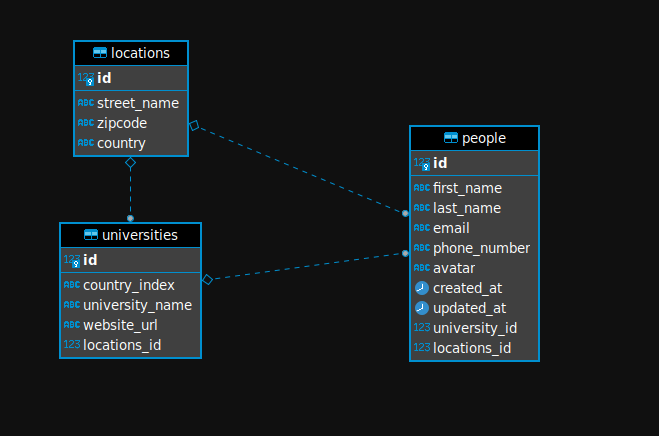
\includegraphics{database_model_dbeaver}
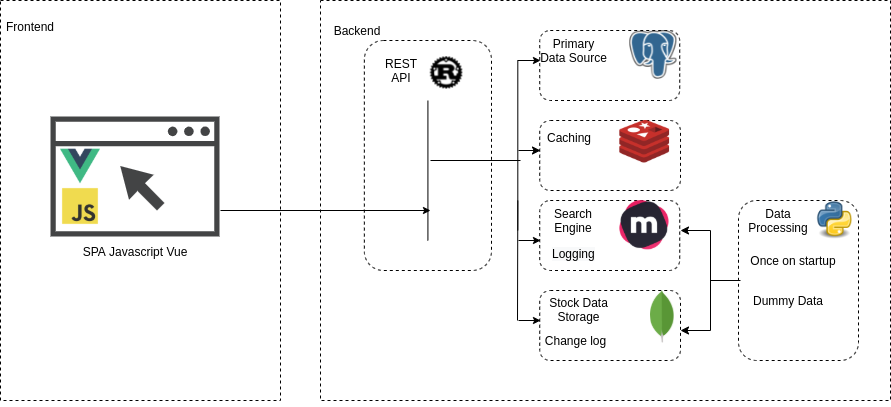
\includegraphics[scale=0.55]{full_application_structure_cropped}
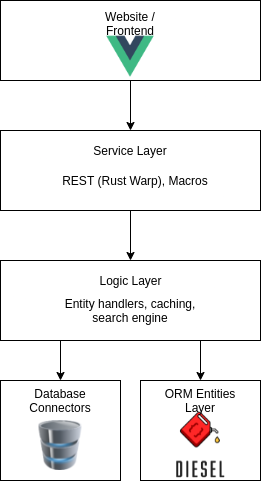
\includegraphics{structure_model_2}


\end{document}
